La clase remoto es la encargada del manejo del protocolo de texto Go(gtp), si el modelo desea enviar un mensaje lo debe hacer por esta clase. Como se puede observar en el diagrama servidor y cliente son hijos de remoto; esto se debe a que el proceso de mensajes entrantes y saliente es el mismo en ambos casos, la \'unica diferencia existente es el momento inicial donde se establece la conexi\'on. Para el proceso de los mensajes, tenemos dos cadenas de responsabilidades; una encargada de los mensajes respuestas(los cuales se caracterizan por el inicio con el caracter =) y los mensajes comandos. Estas cadenas procesan dichos mensajes y le informan al modelo, para que el mismo decida como se debe continuar. \\
La versi\'on del protocolo utilizada es la 2, a pesar que el protocolo fue implementado totalmente; para los alcances del trabajo pr\'actico solo se utilizan los comandos m\'as importantes.

\begin{center}
 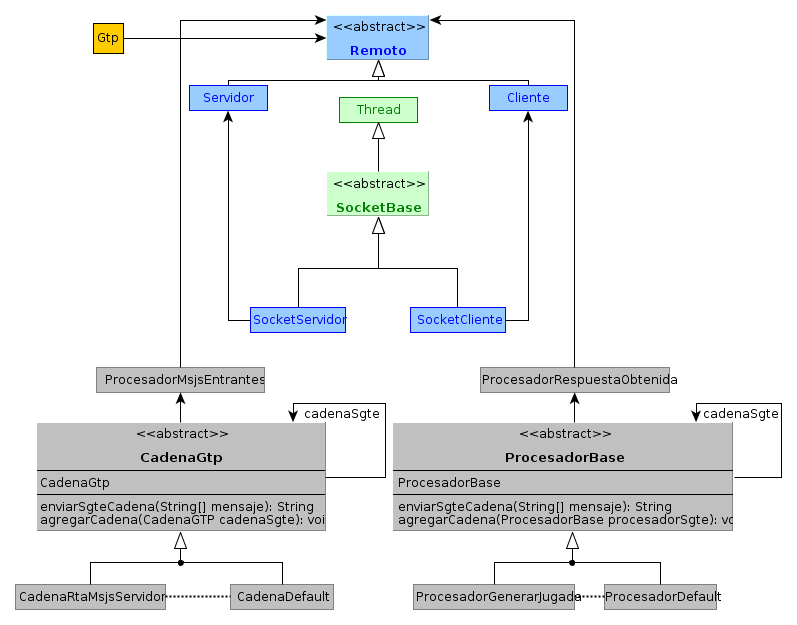
\includegraphics[width=500,height=500]{./Diagramas/DiagramaRemoto/diagrama_remoto.png}
 % diagrama_remoto.png: 797x625 pixel, 72dpi, 28.12x22.05 cm, bb=0 0 797 625
\end{center}
